\sepfootnotecontent{sf:shapeIndexURL}{
   \ifanonymous
      \url{https://anonymous.4open.science/w/shape-index-specification-707E}
   \else
      \url{https://constraintautomaton.github.io/shape-index-specification/}
   \fi
}

\sepfootnotecontent{sf:recursiveShape}{
   \iffalse
    In this paper we ignore ``inverse constraints'' such as
    inverse triple constraint in ShEx 
    %\url{https://shex.io/shex-primer/index.html\#inverse-properties}
    and SHACL Inverse Paths 
    %\url{https://www.w3.org/TR/shacl\#property-path-inverse} 
    to a avoid recurse 
    shape schemas~\cite{Corman2019}.
    We also ignore negative statement.
    \fi
    We only consider shapes that can be transformed into a single \texttt{SELECT} SPARQL query~\cite{Corman2019}.
}

\sepfootnotecontent{sf:subwebsep}{
   We assume an implicit conversion between the subweb specification and the formalization of reachability criteria.
   Space constraints prevent us from detailing the conversion.
}

\sepfootnotecontent{sf:ssf_project}{
   The paper \citetitle{delva2023} additional material also proposes a script to convert SHACL shapes into SPARQL queries.
   \url{https://github.com/MaximeJakubowski/ssf_project}
   \rt{This footnote seems unnecessary, since delva2023 is already cited.}
}


\section{Approach}\label{sec:approach}

This section defines result-based completeness in LTQP, introduces shape indexes, and shows how they enable pruning via a query-shape subsumption algorithm.

To illustrate this approach, we present the example in Figure~\ref{fig:dkg}, which depicts a network of three social media user subwebs, each with its own shape index, as well as resources located outside these subwebs.
The feature query aims to retrieve posts from Subweb~3, along with all associated replies.
Our pruning strategy allows the query engine to explore only the relevant parts of the network, guided by the shapes associated with the resources and the structure of the query.
The process begins with the engine dereferencing the shape index of Subweb~3 and performing a query-shape subsumption check, which determines that only resources containing posts needs to be accessed in this subweb.  
It then checks the shape index of Subweb~1 due to the existing link towards it, where the subsumption check reveals no resources relevant to the query.  
Next, it examines the shape index of Subweb~2 and identifies resources containing comments (i.e., replies) which are relevant.  
Finally, the engine dereferences all reachable resources outside the subwebs that are linked to these relevant comments.

\begin{figure*}
    \centering
    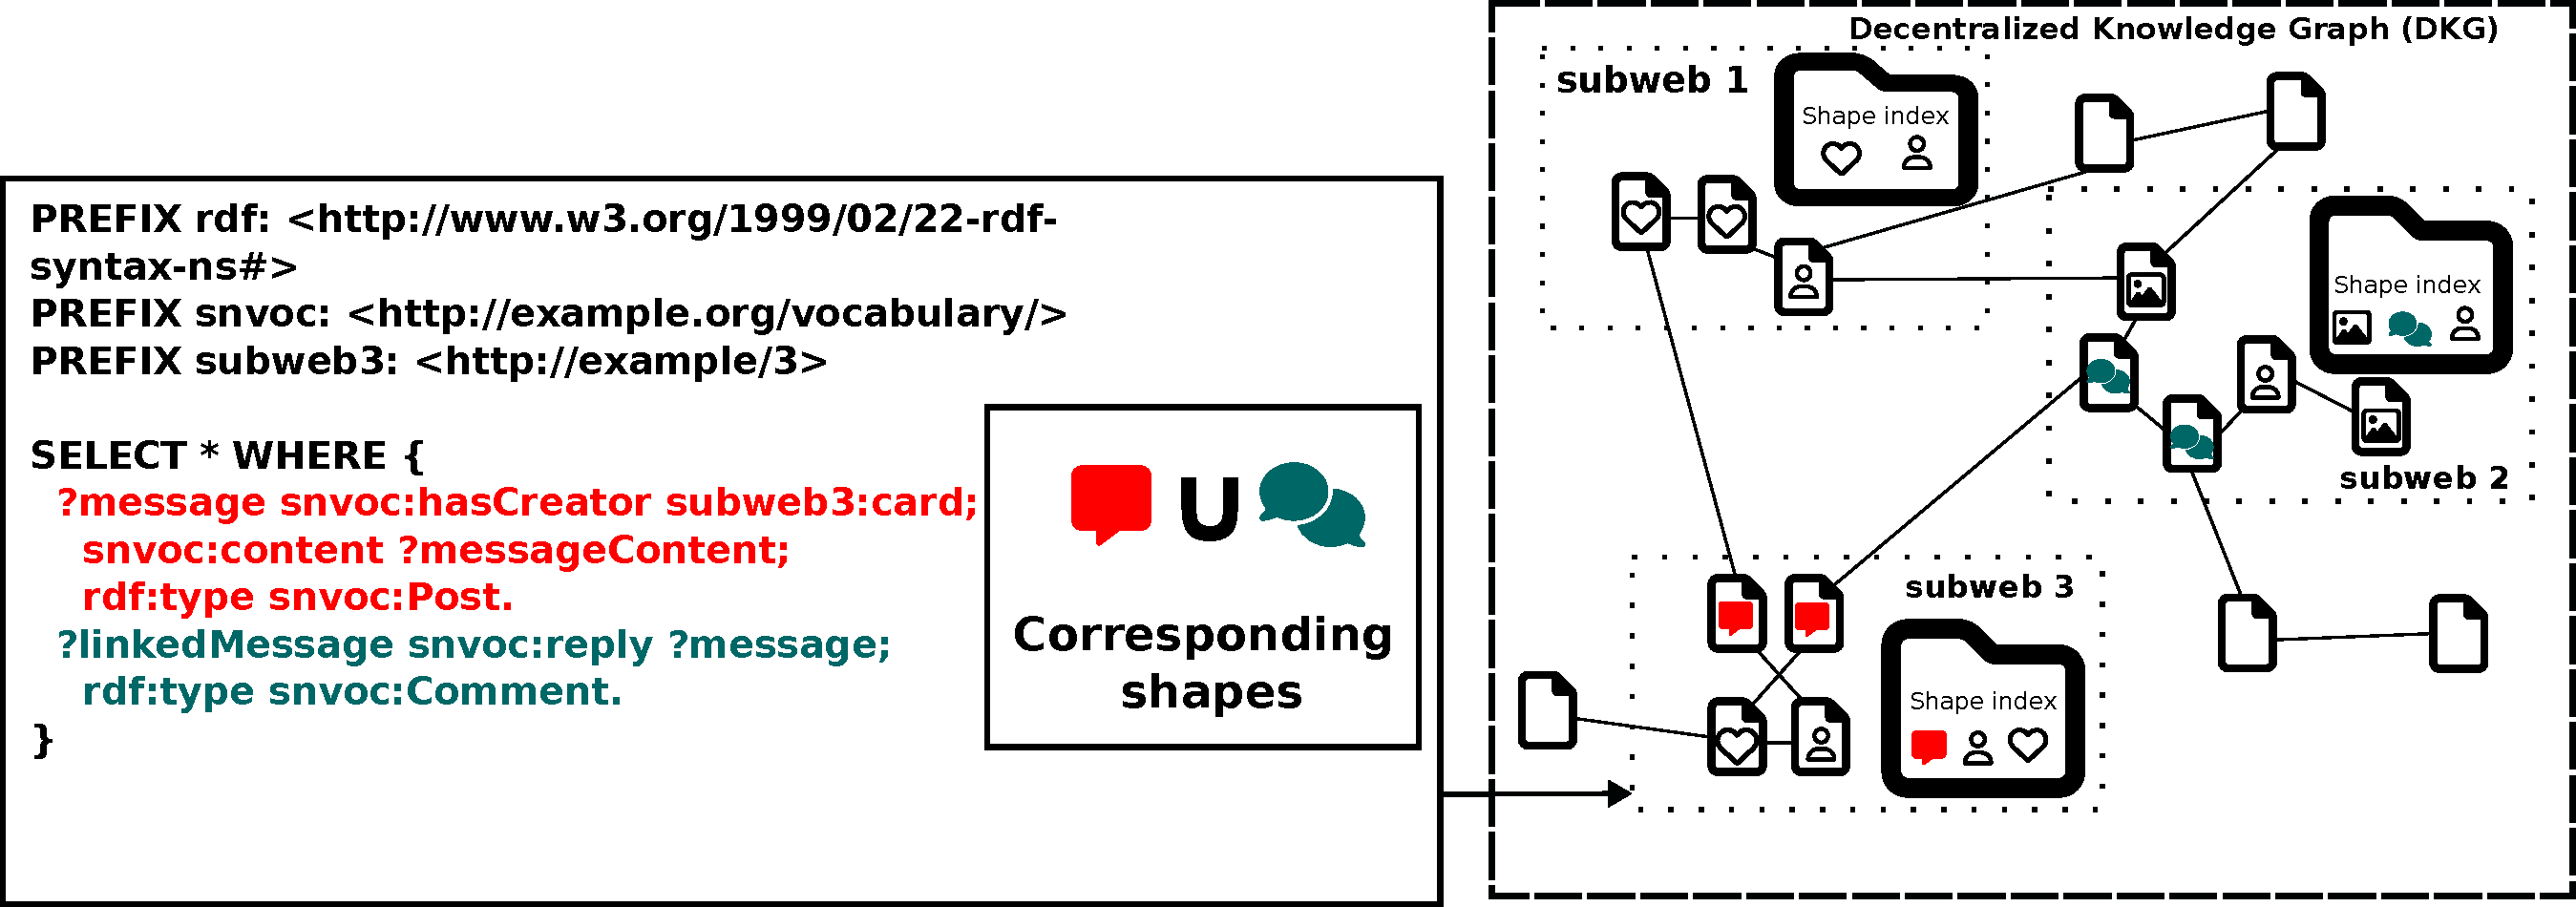
\includegraphics[width=1.0\linewidth]{figure/dkg.pdf}
    \caption{
    When resources of a DKG are indexed with a shape index, a query engine can dereference a subset of the network.
    The nodes represent RDF resources, while the edges represent IRIs linking one resource to another.
    Each subweb has a shape index that maps shapes, represented by icons, to RDF resources by embedding the icon within the node.
    The query engine starts its query at Subweb~3, and the relevant query resources in a subweb are identified with a black node.
    }
    \label{fig:dkg}
\end{figure*}

\subsection{Result-Based Completeness in LTQP}\label{sec:slde}

Our approach of pruning in LTQP focuses on ensuring result completeness, assuming traversal completeness is already defined using reachability criteria.
By concentrating on result completeness, we explore strategies to optimize the search space of link traversal queries through pruning of irrelevant resources.
We formalize result-based completeness in LTQP as follows.
A query is executed over a DKG $G$ formed by the union of all the $g$ in a network $R$.
The query engine has to build a KG $G^{\prime}$ using a reachability criterion $C^{\prime}$ in its internal data store from the KGs $g$ by dereferencing resources $iri \mapsto_{\mathcal{R}} r \in R$.
We formulate an optimization problem to minimize the size of $G^{\prime}$, where the query engine constructs a knowledge graph $G^{\prime\prime} \subseteq G^{\prime}$, potentially smaller, by defining a reachability criterion $C^{\prime\prime}$.
We focus on maintaining the same result completeness, so when using $C^{\prime\prime}$ the following equation must hold

\begin{equation}\label{eq:evalQueryStructuralAssumption}
   [\![ Q ]\!]^{G^{\prime\prime}} = [\![ Q ]\!]^{G^{\prime}}
\end{equation}
for any network $R$.
Since each $g \in G^{\prime\prime}$ is obtained by dereferencing resources $r \in R$, a smaller $G^{\prime\prime}$ compared to $G^{\prime}$ implies that fewer HTTP requests were needed to answer the query. 
Query execution is generally faster with a smaller KG instance, and HTTP requests, being slow and unpredictable~\cite{hartig2016walking}, can dominate execution time. 
Therefore, reducing HTTP requests provides a twofold benefit: fewer resources to process and faster query execution.


\subsection{Shape Index}

\begin{figure*}
   \centering
   % First figure
   \begin{minipage}[t]{0.50\linewidth}
      \centering
      \lstinputlisting[basicstyle=\normalsize\ttfamily]{code/shape_index.nq}
   \end{minipage}
   %\hspace{0.05\textwidth}
   % Second figure
   \begin{minipage}[t]{0.45\linewidth}
      \centering
      \lstinputlisting[basicstyle=\normalsize\ttfamily]{code/gps.rq}
   \end{minipage}

   % General caption
   \caption{
      On the left, an example illustrates a shape index that maps a set of IRIs, represented using a URI template~\cite{ietf6570Template}, to a user shape, and a specific IRI to a post shape.
      On the right, an example illustrates of a graph star pattern where the main subject is \texttt{?comment} and is linked to the \texttt{?message} and \texttt{?forum} star patterns.}
   \label{fig:shapeIndex}
\end{figure*}

Pruning in LTQP requires knowledge of the data models of dereferenced resources.  
However, obtaining complete, up-to-date, and detailed information for each resource in a large decentralized network is impractical.  
To address this, we introduce the \emph{shape index} as a mapping between RDF document sets and RDF data shapes that describes a subweb controlled by a data provider.  
Unlike triple statistics, shapes are independent of the KG's size or updates that remain compliant, making them a more cost-effective solution for use cases with stable data models. 

We formalize a shape index as follows:

\begin{equation}\label{eq:shapeIndex}
   SI = \left\{ s_1 \mapsto \mIRI_1 s_2 \mapsto \mIRI_2 \cdots, s_n \mapsto \mIRI_n \right\}
\end{equation}
where $s_i$ is a shape and $\mIRI_i$ is a set of IRI given $n$ entries.
The subweb described by the index is defined by $D_{SI} = \bigcup_{\mIRI \in \text{codomain}(SI)} \mIRI$.
%A shape index \emph{must} map every resource in $D_{SI}$.
We denote a shape index as \emph{complete} when every shape $s_i \in \text{dom}(SI)$ has a closed world assumption~\cite{Gayo2018b, Gayo2018}~\footnote{We also refer to those shapes as closed.} or \emph{incomplete} otherwise.
A mapping between a shape and a set of IRIs has implications in the distribution of the data in $D_{SI}$.
When a shape $s$ is mapped to an $\mIRI$, then the KG targeted by the mapping, $G = \left\{ g \mid \forall iri \in D_{SI} (\miri \mapsto_{\mathcal{R}} r \land r \mapsto_{\mathcal{G}} g) \right\}$, satisfies $s$.
Given that the shape is closed, then every set of triples in the resource mapped to an $\miri \in D_{SI}$ satisfying the shape must be in a resource mapped to an $\miri \in IRI$.
We provide a complete description of the shape index in an online specification~\sepfootnote{sf:shapeIndexURL} and an example of serialization in Figure~\ref{fig:shapeIndex}.

RDF data shapes use \emph{targets} to identify the set of nodes or entities in a KG to validate.  
In this work, we assume all entities in a KG associated with a shape index follow the same RDF data shape.  
We call these entities graph stars, an extension of the RDF star patterns concept~\cite{Karim2020}.  
Defined in Definition~\ref{def:starPattern}, graph star(s) (patterns)  serve two purposes:
defining targets for validation and capturing relationships between triple patterns and shape entities.  
Star patterns consist of triples with the same subject.
We extend this concept by linking star patterns such that the objects of triples in one star pattern act as subjects in others, forming a graph structure.
For example, a user linking to their posts with recursive replies can be captured with a root star pattern for the user and nested patterns for the posts and replies.  
Thus, the targets of the shapes in the shape index correspond to the subject of each root star pattern when a KG is divided into graph stars with no shared partial graph stars.  
Figure~\ref{fig:shapeIndex} illustrates an example of a graph star pattern.

\begin{definition}[Star Pattern]
   Given a query $Q$, we define a star pattern $Q_{star}$ as a set of $tp \in Q$~\cite{Karim2020} with the same subject such that 
   given a builder function 
   \begin{equation}
       BQ_{star}(s) = \left\{ tp_i \in Q \mid S(tp_i) = s \right\}
   \end{equation}
   with $s \in \mathcal{I}\mathcal{B}\mathcal{V}$ then $Q_{star} = BQ_{star}(s)$.

\end{definition}

\begin{definition}[Graph Star Pattern (GSP) and Graph Star]\label{def:starPattern}
   
   We define a GSP $Q_{starG}$ as the union between a root star pattern $Q_{star_s}$
   and the star patterns having as subject term an object term of another star pattern in $Q_{starG}$.
   We define a function 
   $O_{star}: q \in Q \rightarrow  (\mathcal{I}\mathcal{B}\mathcal{V})^2$
   that returns every non-literal object terms of a star pattern.

   We then define $Q_{starG}$ given a  set of partial GSP $Q_{starGT}$
   \begin{equation}
      Q_{starG} = \bigcup_{q \in Q_{starGT}} q
   \end{equation}
   where $Q_{starGT}$ is formed with a root $Q_{star_s}$ by

   \begin{equation}
           q_i =
       \begin{cases}
         \left\{ Q_{star_s} \right\} & \text{if } i = 1 \\
           \left\{ BQ_{star}(o) \mid o \in \bigcup_{q \in Q_{starGT_{i-1}}} O_{star}(q) \right\} & \text{if } i>1
       \end{cases}
   \end{equation}

   We also define a function  
   $S_{star}: q \rightarrow  \mathcal{I}\mathcal{B}\mathcal{V}$
   returning the subjects of the $q_i$ of a $Q_{starG}$.

   We propose a similar definition for the context of KGs where we replace the query $Q$ by a KG $G$. 
   We denote this structure a graph star.
   
\end{definition}

\subsubsection{Practical Considerations for Shape Indexes}

The construction and maintenance of shape indexes are beyond the scope of this work. 
Although not evaluated here, shape indexes seem to require less effort to generate than VoID descriptions~\cite{Boehm2011}, as they do not include detailed statistics such as triple counts. 
Nonetheless, VoID descriptions have been successfully employed for query optimization in federated queries~\cite{Montoya2017}. 

Exposed schemas can also enhance interoperability, which is important in many application domains~\cite{rowland2022interoperability, solidSolidApplication, binding2016improving, roller2015benefits}. 
Thus, data publishers may have incentives to expose a shape index not only to improve query engine performance but also to satisfy other domain-specific requirements.

RDF data shapes can be prescriptive or descriptive.
For descriptive shape indexes, automatic RDF data shape generation methods~\cite{fernandez2023extracting} can facilitate their creation. 
Entries in shape indexes correspond to sets of IRIs, which can be structured using URI templates~\cite{ietf6570Template}, reducing the need for exhaustive redefinition. 
For prescriptive shapes, contributions in shape-based data integration~\cite{LabraGayo2023} can help prevent the generation of invalid resources.

Overall, shape indexes are lightweight metadata that can be maintained with relatively low effort, especially compared to statistical summaries such as VoID.
Publishing them not only benefits query optimization but also contributes to FAIR data principles~\cite{Wilkinson2016} by enhancing machine-actionability and interoperability.
Future work should investigate construction and maintenance strategies for shape indexes in practical deployment scenarios.

\subsection{Link Pruning Using Shape Indexes}\label{sec:sourceSelection}

In this section, we establish the connection between shape indexes and link pruning in LTQP as a means to reduce the search domain.
In our method, rather than traversing the entire DKG $D$ associated with a shape index, the engine traverses a subgraph $D^{\prime} \subseteq D$, effectively ignoring resources that are knowably irrelevant to the query.
%The concept of composite reachability criteria allows us to ignore certain sources during traversal based on the knowledge acquired during traversal.
Our approach involves dynamically constructing new reachability criteria during traversal that are more selective as we discover and analyze shape indexes.
These criteria are designed so that they will always produce the same completeness of results as the one that was defined at the beginning of the traversal.

\iffalse
\rt{I still think introducing time here is a really bad idea. I'm almost certain that reviewers will shoot the paper down because of this. In the formalization, let's just assume prior knowledge of all shape indexes and corresponding reachability criteria. Combining them during query execution is an implementation detail.}
More formally, let us introduce time $t$ as a factor for our reachability criteria $C_t$.
The query execution begins with an initial reachability criterion $C_0$.
At any time $t$, Equation~\ref{eq:evalQueryStructuralAssumption} must hold if we consider $C_t = C_{t+1} = C_{t+2} \dots = C_{tf}$ until the end of the execution $tf$, given that $G^{\prime}$ is produced using $C_0$.
\fi

To define more selective reachabilities, we propose extending the reachability criteria by formalizing a chain of criteria in a concept called \emph{composite reachability criteria}.
In this form, a reachability criterion $cp_i$ is said to \emph{prune} links, and $cd_i$ is said to \emph{discover} links.
Equation~\ref{eq:cReachabilityCriteria} formalizes a composite reachability criterion $C$.
where $Cd$ is the set of every $cd_i(t, iri, Q)$ and $Cp$ the set of every $cp_i(t, iri, Q)$ used by the engine.

\begin{equation}\label{eq:cReachabilityCriteria}
   C(t, iri, Q) = \bigvee_{cd \in Cd} cd(t, iri, Q) \mathrel{\land} \bigwedge_{cp \in Cp} \, cp(t, iri, Q)
\end{equation}

To perform pruning in LTQP with shape indexes, an initial reachability criterion $C_0$ is defined.
This criterion must include a discovery reachability criterion $cd_{\text{shape index}}$ that leads to a shape index document.  
After dereferencing a shape index $SI_i$, the query engine creates a set of links $IRI_p$ containing the links to prune.  
The links to prune are identified by evaluating the shape index to find IRIs that are not relevant to the query, such that Equation~\ref{eq:evalQueryStructuralAssumption} holds, given that $G^{\prime}$ is produced using $C_0$.  
This is done by performing a query-shape subsumption check ($\sqsubseteq_{qs}$), defined in the next section.

We define, given a query $Q$,
$$
IRI_p = \left\{ \bigcup SI_i(s_j) | Q \sqsubseteq_{qs}  s_j = \mathrm{false} \land s_j \in \text{dom}(SI_i) \right\}
$$
From this sets of links we define a pruning reachability criteria;
\begin{equation}
       cp_{si}(t, iri, Q) = iri \notin IRI_p
\end{equation}
The new reachability $C_i$ is created by taking the $Cd$ and $Cp$ of $C_{i-1}$ and adding $cp_{si}$ to $Cp$.

This approach has three main limitations.  
First, it assumes that data providers maintain up-to-date shape indexes; outdated indexes may lead to incomplete results.
A similar criticism could be leveraged against the method exploiting VoID descriptions~\cite{Montoya2017}.
Second, if the query-shape subsumption check requires dereferencing all documents, it becomes ineffective and may slow down query execution.  
Third, the approach does not consider cases where querying irrelevant documents could uncover relevant ones via additional reachability criteria.  
Addressing this would require translating these criteria into queries, which is beyond the scope of this paper.

\subsection{Query-Shape Subsumption}\label{sec:containment}

To determine whether the contents of a resource conforming to a shape is query-relevant, we define a \emph{query-shape subsumption} problem denoted as $Q \sqsubseteq_{qs} S$, meaning $Q$ is subsumed by $S$.
A common approach for validating shapes over an RDF graph is to translate shapes into SPARQL queries~\sepfootnote{sf:recursiveShape}~\cite{labragayo2017validatingdescribinglinkeddata, Corman2019, spapeExpressionConvert, delva2023}.
We denote the transformation of a shape $S$ into a query as $T(S)$, which yields a query $Q_s$.
We transform open shapes as queries over the entire KG, since they impose only the minimal constraints required of a KG.
When the problem is expressed as $\text{GSP} \sqsubseteq_{qs} Q_s$, we say that a GSP is subsumed by $S$ if every result of the GSP can be extended to a result of $Q_s$, and every triple pattern in a GSP is equivalent to or a specialization of those in the $Q_s$.
Thus, the problem diverges from traditional query containment and query subsumption~\cite{Spasi2023, Pichler2014} under set semantics. 
Query-shape subsumption does not consider only the set of solution mappings but also the constraints of the queries.
\footnote{In this sense, it bears some similarity to query containment under bag semantics, particularly through the notion of ``goals-onto'' containment mappings~\cite{Chaudhuri1993, Afrati2010}.} 
The complexity of the problem is reduced by the fact that $Q_s$ has a GSP structure where predicates are always IRIs.
This structure arises because shapes describe constraints on predicate and object terms of sets of triple.
By exploiting this structure, it is possible to design an algorithm with polynomial-time complexity.
Moreover, empirical studies suggest that real-world queries tend to be relatively small~\cite{Doan2012, Bonifati2019}, making this algorithm applicable in practice.

More formally, for a $S$ to subsume a shape GSP, we consider the queries $Q$ and $Q_s$, where $Q_s$ is the query translated from $S$, and both are of the form 
$$
Q_i = Q_{\text{body}} \bowtie Q_{\text{unions}}
$$
where $Q_{\text{body}}$ denote the Basic Graph Pattern (BGP) of the query, and 
$Q_{\text{unions}} = \bigcup Q_u$ represent the Union Graph Patterns (UGPs)~\cite{w3SPARQLQuery} expressed in normal form, meaning 
each $Q_u$ is of the form $q_i \cup q_j$, where each $q$ is a BGP contain no union statements.

\subsubsection{Algorithm}

\input{time-complexity/algorithm/subsums_q_star}

We define the function $subsums_{\text{graph star}}$ in Algorithm~\ref{alg:containmentTree} to evaluate whether a GSP with a root star pattern $Q_{star_i}$ from $Q_{starG_i}$ is sumbsumed by $Q_s$. 
The algorithm also takes a set $Eval_{star}$ to track which partial graph star patterns have already been evaluated.
The algorithm iterates over each triple pattern in the root star pattern $Q_{star_i}$ and uses the $match$ function to check if there exists a triple pattern in the BGP of $Q_s$ whose domain of matched triples is a superset of that of the current pattern.
If the triple pattern cannot be found in the BGP, the algorithm then looks into the UGPs of $Q_s$. 
%Since we assume that the union statements are not nested, this limits the number of recursive calls.
If an equivalent triple pattern is found, the algorithm checks whether the object of the triple pattern is the subject of a partial graph star pattern in $Q_{starG_i}$.
In this case, the algorithm recursively applies the same procedure to this partial GSP.
To avoid cycles and redundant evaluations we maintain a set of evaluated answers in $Eval_{star}$.
\iffalse
We notice that the complexity of Algorithm~\ref{alg:containmentTree} is $O(n_{tp}^2 \cdot n_{sunion})$
where $n_{tp}$ is the number of triple patterns of $Q_{starG_i}$ and $n_{sunion}$ the number of UGP in $Q_s$.
\fi
To solve $Q \sqsubseteq_{qs} S$, we need to consider the number of GSP from the BGP with their number of segments in the UGP and the number of BGPs in the UGPs.
This procedure is detailed in Algorithm~\ref{alg:containmentQuery}.
%This operation results again in a polynomial time complexity algorithm.
The following paragraphs analyze the time complexity of the algorithm.
%Additional analyses of the algorithms are available in the \hyperref[sec:supplementalMaterial]{supplementary material}.
%To solve $Q \sqsubseteq_{qs} S$, we need to consider the $n_{starG}$ graph star from the BGP with their $n_{starGu}$ segment in the UGP and $n_{starGui}$ BGP in the UGP.
%This operation results in a polynomial time complexity of $O(n_o \times n_{tp}^2 \times n_{union}^2 \times n_{starG} \times n_{starGu} \times n_{starGui})$.
%In the \nameref{sec:appendix} Algorithm~\ref{alg:containment} present the full resolution to evaluate each graph star pattern.

\subsubsection{Time Complexity Analysis}

\paragraph{Worst-case per $Q_{star}$}
Let $n_{qstar}$ denote the number of distinct $Q_{star} \in Q_{starG_i}$.
For each node $Q_{star}$, the algorithm iterates over its triple patterns (line 4 to 25), resulting in a time complexity of $O(n_{tp_{Q_{star}}})$.
For each triple pattern that does not match the shape body ($Q_{s\mathrm{body}}$), the algorithm iterates over all union branches in $Q_{sunion}$ (line 7 to 11), making at most $n_{sunion}$ recursive calls.
The algorithm traverses the $q_{us}$ graph however each $q_{us} \in Q_{sunion}$ cannot contain a Union Graph Pattern (UGP), and is therefore always of the form $Q_s = Q_{s\mathrm{body}}$, making this 
branch (line 5 to 15) of the algorithm after a first execution not the worst case with a complexity of $O(n_{tp_{Q_{star}}}^{2} \cdot n_{sunion})$.

After the first execution, the worst-case scenario becomes one in which the triple patterns matches a pattern in $Q_{s\mathrm{body}}$, and the condition $O(tp) \in S_{star}(Q_{starG_i})$ holds (line 17 to 22).
In such cases, the algorithm recursively explores the corresponding partial Graph Star Pattern (GSP) by executing $subsums_{\mathrm{graph star}}$, following a graph traversal paradigm.


\paragraph{Tree Traversal Argument}
Although $Q_{starG_i}$ is a graph, the algorithm avoids cycles due to "caching", once a node $Q_{star}$ is evaluated, its result is stored in $Eval_{star}$.
Therefore, each node is visited at most once, and the overall traversal is equivalent to a tree traversal of size $n_{qstar} \leq |Q_{starG_i}|$.

\paragraph{Total Complexity}
Let $n_{tp_{Q_{star}}}$ denote the number of triple patterns in a particular $Q_{star}$, and let $n_{tp}$ be the total number of triple patterns across all nodes, so
$$
n_{tp} = \sum_{Q_{star} \in Q_{starG_i}} n_{tp_{Q_{star}}}
$$

Then the total number of recursive operations over all nodes is bounded by:
$$
O\left(\sum_{i=1}^{n_{qstar}} n_{sunion} \cdot n_{tp_{Q_{star_i}}}^{2}\right)
$$

$$
O\left(n_{sunion} \cdot \sum_{i=1}^{n_{qstar}} n_{tp_{Q_{star_i}}}^{2}\right)
$$

$$
O\left(n_{sunion} \cdot \left(n_{tp}^{2} - \sum_{i=1, j=1, i \neq j}^{n_{qstar}}  n_{tp_{Q_{star_i}}} \cdot  n_{tp_{Q_{star_j}}}\right)\right)
$$

$$
O\left(n_{sunion} \cdot n_{tp}^{2}\right)
$$

\paragraph{Time Complexity of the $subsums_{\mathrm{Q}}$ Algorithm}

\input{time-complexity/algorithm/subsums_Q}

The time complexity of the $subsums_{\mathrm{Q}}$ algorithm is straightforward to derive, as it consists of iterating over the GSP of the query and applying the $subsums_{\mathrm{graph star}}$ algorithm. Thus, the time complexity is given by:
\begin{equation}
O\left(n_{sunion} \cdot n_{tp_{max}}^{2} \cdot n_{Q_{star_{max}}} \cdot n_{Q_{starG}}\right)
\end{equation}

Where, $n_{tp_{max}}$ is the maximum number of triple patterns in any $Q_{starG}$,
$n_{Q_{star_{max}}}$ is the maximum number of $Q_{star}$ patterns in any $Q_{starG}$, and
$n_{Q_{starG}}$ is the number of Graph Pattern Structures (GPS) in the query $Q$.\footnote{
    Sharing the evaluation results $Eval_{star}$ from $subsums_{\mathrm{graph star}}$ could reduce execution time and potentially the algorithm's complexity.
}
